\documentclass[review]{elsarticle}

\usepackage{lineno,hyperref}
\usepackage{epstopdf}
\usepackage{comment}
\usepackage{subcaption}
\usepackage{color}
\usepackage{lipsum}
\usepackage{multicol}
\usepackage{amssymb}
\usepackage{amsmath}
\usepackage{bm}
\usepackage{amsfonts}
\usepackage{multirow}
\usepackage{graphicx}
\usepackage{mathtools, amssymb}
\usepackage{CJK}
\usepackage{graphicx}
\usepackage{epsfig}
\usepackage{float}
\usepackage{multirow}
\usepackage{algorithm}
\usepackage{algorithmic}
\usepackage{indentfirst}
\usepackage{booktabs}
\usepackage{amsmath}
\modulolinenumbers[5]
%\journal{Journal of \LaTeX\ Templates}

%%%%%%%%%%%%%%%%%%%%%%%
%% Elsevier bibliography styles
%%%%%%%%%%%%%%%%%%%%%%%
%% To change the style, put a % in front of the second line of the current style and
%% remove the % from the second line of the style you would like to use.
%%%%%%%%%%%%%%%%%%%%%%%

%% Numbered
%\bibliographystyle{model1-num-names}

%% Numbered without titles
%\bibliographystyle{model1a-num-names}

%% Harvard
%\bibliographystyle{model2-names.bst}\biboptions{authoryear}

%% Vancouver numbered
%\usepackage{numcompress}\bibliographystyle{model3-num-names}

%% Vancouver name/year
%\usepackage{numcompress}\bibliographystyle{model4-names}\biboptions{authoryear}

%% APA style
%\bibliographystyle{model5-names}\biboptions{authoryear}

%% AMA style
%\usepackage{numcompress}\bibliographystyle{model6-num-names}

%% `Elsevier LaTeX' style

\bibliographystyle{elsarticle-num}
%%%%%%%%%%%%%%%%%%%%%%%

\begin{document}

\begin{frontmatter}
\title{Competition Updating Rules of Social Opinions on Two Layer Networks}
%\tnotetext[mytitlenote]{Fully documented templates are available in the elsarticle package on \href{http://www.ctan.org/tex-archive/macros/latex/contrib/elsarticle}{CTAN}.}

%% Group authors per affiliation:
\author[mymainaddress,mysecondaryaddress]{Cho Hyunchel}
\author[mymainaddress,mysecondaryaddress]{Wang Lin\corref{mycorrespondingauthor}}
\cortext[mycorrespondingauthor]{Corresponding author}
\ead{wanglin@sjtu.edu.cn}
\address[mymainaddress]{Department of Automation, Shanghai Jiao Tong University, Shanghai 200240, P. R. China}
\address[mysecondaryaddress]{Key Laboratory of System Control and Information Processing, Ministry of Education of China, Shanghai 200240, P. R. China}

\begin{abstract}
Social conflict usually can be investigated based on the competition of two-layers network. Two-layers network has individual dynamics and updating rule on each layer. In this article, a competition model is studied on interconnected networks with two-layer opinions, where the first layer represents social opinion formation and the second layer makes decision such as the congress or leader. Starting with a polarized competition case where layer A has all the positive opinion and layer B has all the negative opinion, two layers have mutual interaction. Here, we focus on the way how two layers update their states, especially time-related updating rules. It is researched that there has an influence on states of two-layers network by controlling updating rules. Updating rules are divided into 3 categories, sequential order, simultaneous order and random order. Considering all cases, 25 updating rules are simulated, which shows that sequential order makes it easy to reach consensus for social opinion, and simultaneous order makes it hard to reach consensus and sometimes makes transition to coexistence or opposite orientation. In real world, the order of dynamics would be analyzed as the decision-making method, interaction method between nodes, and the characteristics of nodes. 

\end{abstract}

\begin{keyword}
Interconnected Networks \sep Opinion Dynamics\sep Decision Making \sep Updating Rules
%\MSC[2010] 00-01\sep  99-00
\end{keyword}

\end{frontmatter}
\linenumbers

\section{Introduction}
Social conflicts and consensus are very important issues in real world. Social conflicts and consensus happen in various ways. Voting, or adoption of new policies can be also seen as a kind of social conflicts and consensus. They are widely recognized that opinion formation has conflict with decision making formation and they are in competition for their opinions. This competition can be considered as interaction on interconnected networks\cite{bianconi2018,domenico2013,tomasini2015,kimsangwoo2012,newman2010,boccaletti2014,mikko2014,fangwu2004}. 

Many researchers have studied many techniques for modeling and analyzing competition on opinion dynamics\cite{amato2017,quattrociocchi2014,haibo2017, hua2014}, voter model\cite{redner2017}, game theory\cite{smyrnakis2019} and many more\cite{danziger2019,namkhanhvu2017,laguna2004,masuda2014,zuev2012, shenyu2018, zhou2018}.  For competition of interconnected networks, many researches have been performed in the various networks, for example the dissemination of computer viruses, messages, opinions, memes, diseases and rumors\cite{hua2014,shenyu2018, zhou2018, alvarez2016,gomez2015,diep2017,rocca2014,velasquez2018}. Opinion dynamics on two-layer or multi-layer networks have been investigated, based on \textit{Abrams-Strogatz(AS)} model\cite{abrams2003,vazquez2010} and \textit{M} model\cite{rocca2014}. Existing researches mainly have focused on what conditions all agents reach a consensus or dissent, which have shown that the system can make positive consensus, negative consensus or coexistence under certain range of volatility, reinforcement, or prestige. Also, the thresholds or critical points for transition are found to explain and analyze the social phenomena in real world such as the legislation, election result, and social network\cite{amato2017, alvarez2016, diep2017}. In \cite{gomez2015}, it is shown that the transition from localized to mixed status occurs through a cascade from poorly connected nodes in the layers to the highly connected ones. In addition, the main features, such as transition and cascade, found in Monte Carlo simulation are exactly characterized by the mean-field theory and magnetization\cite{amato2017, alvarez2016, gomez2015, diep2017}.   

For further understanding the competition on two-layer network, it is very important to investigate the interaction between nodes or layers. Methods of interaction between nodes are very various.\cite{sirbu2017} But, related to time, the types of interactions  would be divided into two categories, simultaneous interaction and sequential interaction. In economics and social networks, it has been proven that there exists different results between simultaneous and sequential interactions.\cite{hoffman2011, dietrich2004} In \cite{hoffman2011}, it was researched that how experimental subjects update exogenously induced prior information when receiving two information signals simultaneously versus receiving the same signals sequentially. As the experimental results, the simultaneous treatment is very different from sequential treatment, and under sequential information,  subjects’ mean estimates of the two treatments(good news preceding bad news or vice versa) are also significantly different from each other. In conclusion, both sequencing and the order of information processing suggest which one arrives matters. 
And, in \cite{dietrich2004}, the usual random sequential updating rule is replaced  by simultaneous updating on the Sznajd model. As the results, it is found out that this change makes a complete consensus much more difficult. The reason is analyzed as that for simultaneous updating some agents simultaneously receive conflicting messages from different neighbor pairs and thus refuse to change their opinion.
     
Based on these results, we would study the competitions on interconnected networks with various updating rules, and investigate which updating rule has more probability to perform consensus results. With Monte Carlos simulations, the simulation results of various dynamics order models be compared, which shows the vital influence of updating rules. Through these results, it is found out that as the networks have more simultaneous updating rules, it is harder to reach consensus and it sometimes makes transition to opposite state. And we could analyzed that dynamics orders can be considered as decision-making method, communication method, and nodes feature. According to social network conditions, proper dynamics orders could be applied for real networks.      

The paper is organized as follows. In section 2, competition dynamics of interconnected network, that is applied to each layer, is described and presented its features. In section 3, the simulation results of two-layer networks with various updating rules are presented, compared and analyzed. Lastly, in section 4, the simulation results are summarized.


\section{Modeling}
\label{modeling}
The model of interconnected network consists of two layers. Each layer consists of \textit{Barabasi-Albert(BA)} network that has $N$ nodes with attaching new nodes each with $K$ edges that are preferentially attached to existing nodes with high degree as introduced in \cite{barabasi1999}. Each node of one layer is connected with a random node on the other layer. This means each node has only $1$ external un-directed edge. Simulations are preformed on network with $N=2048$, and $K = 3$.

And, each layer has different dynamics. For layer A, the node changes its state according to $M$ model as introduced in \cite{rocca2014}. Here, we choose $M=2$, that each node has four states $(-2, -1, +1, +2)$. For each link $(k, j)$ belongs to layer A,  the dynamics are designed as follows:
\begin{itemize}
	\item Compromise : if two nodes connected with link$(k, j)$ have opposite orientations, their states become more moderate with probability $q$ :
	\begin{align}
	\mbox{if } S_k<0 \mbox{ and } S_j>0  \Rightarrow (S_k, S_j) \rightarrow (S_k^r, S_j^l) \mbox{ with } prob.q,\\
	\mbox{if } S_k>0 \mbox{ and } S_j<0  \Rightarrow (S_k, S_j) \rightarrow (S_k^l, S_j^r) \mbox{ with } prob.q.
	\end{align}
	If $S_k = \pm1$ and $S_j = \mp1$, one switches orientation at random:
	\begin{align}
	(\pm 1, \mp 1)\rightarrow \left\{\begin{matrix}
	(+1, +1) \mbox{ with } prob.q/2,
	\\(-1, -1)\mbox{ with } prob.q/2.
	\end{matrix}\right.
	\end{align}
	\item Persuasion : if two nodes connected with link$(k, j)$ have the same orientation, their states become more extreme with probability $p$ :
	\begin{align}
	\mbox{if } S_k<0 \mbox{ and } S_j<0  \Rightarrow (S_k, S_j) \rightarrow (S_k^l, S_j^l) \mbox{ with } prob.p,\\
	\mbox{if } S_k>0 \mbox{ and } S_j>0  \Rightarrow (S_k, S_j) \rightarrow (S_k^r, S_j^r) \mbox{ with } prob.p.
	\end{align}
\end{itemize}
For each external link $(k,j)$ with $k$ belong to layer A, the state of node $k$ is updated according to :
\begin{itemize}
	\item $S_k \cdot S_j < 0$ :
	\begin{align}
	\mbox{if } S_k<0 \mbox{ and } S_j>0  \Rightarrow (S_k, S_j) \rightarrow (S_k^r, S_j) \mbox{ with } prob.q,\\
	\mbox{if } S_k>0 \mbox{ and } S_j<0  \Rightarrow (S_k, S_j) \rightarrow (S_k^l, S_j) \mbox{ with } prob.q.
	\end{align}
	\item $S_k \cdot S_j > 0$ :
	\begin{align}
	\mbox{if } S_k<0 \mbox{ and } S_j<0  \Rightarrow (S_k, S_j) \rightarrow (S_k^l, S_j) \mbox{ with } prob.p,\\
	\mbox{if } S_k>0 \mbox{ and } S_j>0  \Rightarrow (S_k, S_j) \rightarrow (S_k^r, S_j) \mbox{ with } prob.p.
	\end{align}
\end{itemize}
Here, $S_k^r$ and $S_k^l$ denote the right and left neighboring states of $k$, defined as
\begin{align}
S_k^r &= \left\{\begin{matrix}
+1,\mbox{ for } S_k = -1\\
+2,\mbox{ for } S_k = +2\\ 
S_k + 1,\mbox{ otherwise }, 
\end{matrix}\right. &
S_k^l &= \left\{\begin{matrix}
-1,\mbox{ for } S_k= +1
\\ -2,\mbox{ for } S_k=-2
\\ S_k - 1,\mbox{ otherwise }.
\end{matrix}\right.
\end{align}

The sign of $S^A$ represents its opinion orientation and its absolute value $|S^A|$ measures the intensity of its opinion. So, $|S^A|=2$ represents to a positive or a negative extremist, while  $|S^A|=1$ correspond to a moderate opinion of each side. In case of internal link $(k, j)$ belong to layer A, when the nodes have the same orientation$(S_kS_j>0)$, if the states of nodes are moderate, then they become extreme$(S_k=\pm1 \rightarrow \pm2, S_j= \pm1 \rightarrow \pm2)$ with probability $p$. If they are already extreme, they remain extreme$(S_k=\pm2 \rightarrow \pm2, S_j= \pm2 \rightarrow \pm2)$. On the other hand, when the nodes have opposite orientations$(S_kS_j<0)$, if they are extreme, the states of nodes become moderate$(S_k=\pm2 \rightarrow \pm1, S_j= \pm2 \rightarrow \pm1)$ with probability $q$. If they are already moderate, they switch orientations individually$(S_k=\pm1 \rightarrow \mp1, S_j= \pm1 \rightarrow \mp1)$.  In case of interaction between node in layer A and node in layer B, node in layer A follows opinion dynamics formula, but the state of node in layer B does not change. In other words, the state of layer B affects layer A, but layer A dynamics does not affect the state of node in layer B. For example, one of the layer A node, $S_k = +2$ is connected with  $S_j = -1$ node of layer B. Here, $S_k$ will change into $S_k = +1$ with $prob.q$. But $S_j$ will not change, which indicates that the states of layer B will influence the states of layer A.

The dynamics of layer B follows the decision-making dynamics as introduced in \cite{abrams2003, vazquez2010}. The state of node i in layer B can be $+1$ and $-1$, and it updates according to

\begin{equation}
{P_B}({S_i} \to  - {S_i}) = \begin{cases}
{\left({\displaystyle\frac{{{i_i} + {e_i}}}{{{n^{ - {S_i}}}}}}\right)}{\cdot}{\left({\displaystyle\frac{{n^{-{S_i}}}}{{{i_i} + {e_i}}}} \right)^{1/v}}  ,\mbox{ if } v \ne 0\\
0,\mbox{ if } v = 0\\
0,\mbox{ if } {n^{ - {S_i}}} = 0
\end{cases},
\end{equation}

where $i_i$ is the number of internal edges and $e_i$ is the number of external edges. $n^{-S_i}$ is the number of neighbors of i with opposite state $-S_i$. $v$ represents the volatility that measures how prone a node change its state. The scale of $v$ is from $0$ to $1$. If $v \simeq 0$,  a node is unlikely to change its state. On the other hand, if $v \simeq 1$, a node is very likely to change its state. Also, this formula shows that the more the number of nodes connected with the opposite state is, the easier the nodes are to change into the opposite state.\\
\begin{figure}[!htb]
	\centering
	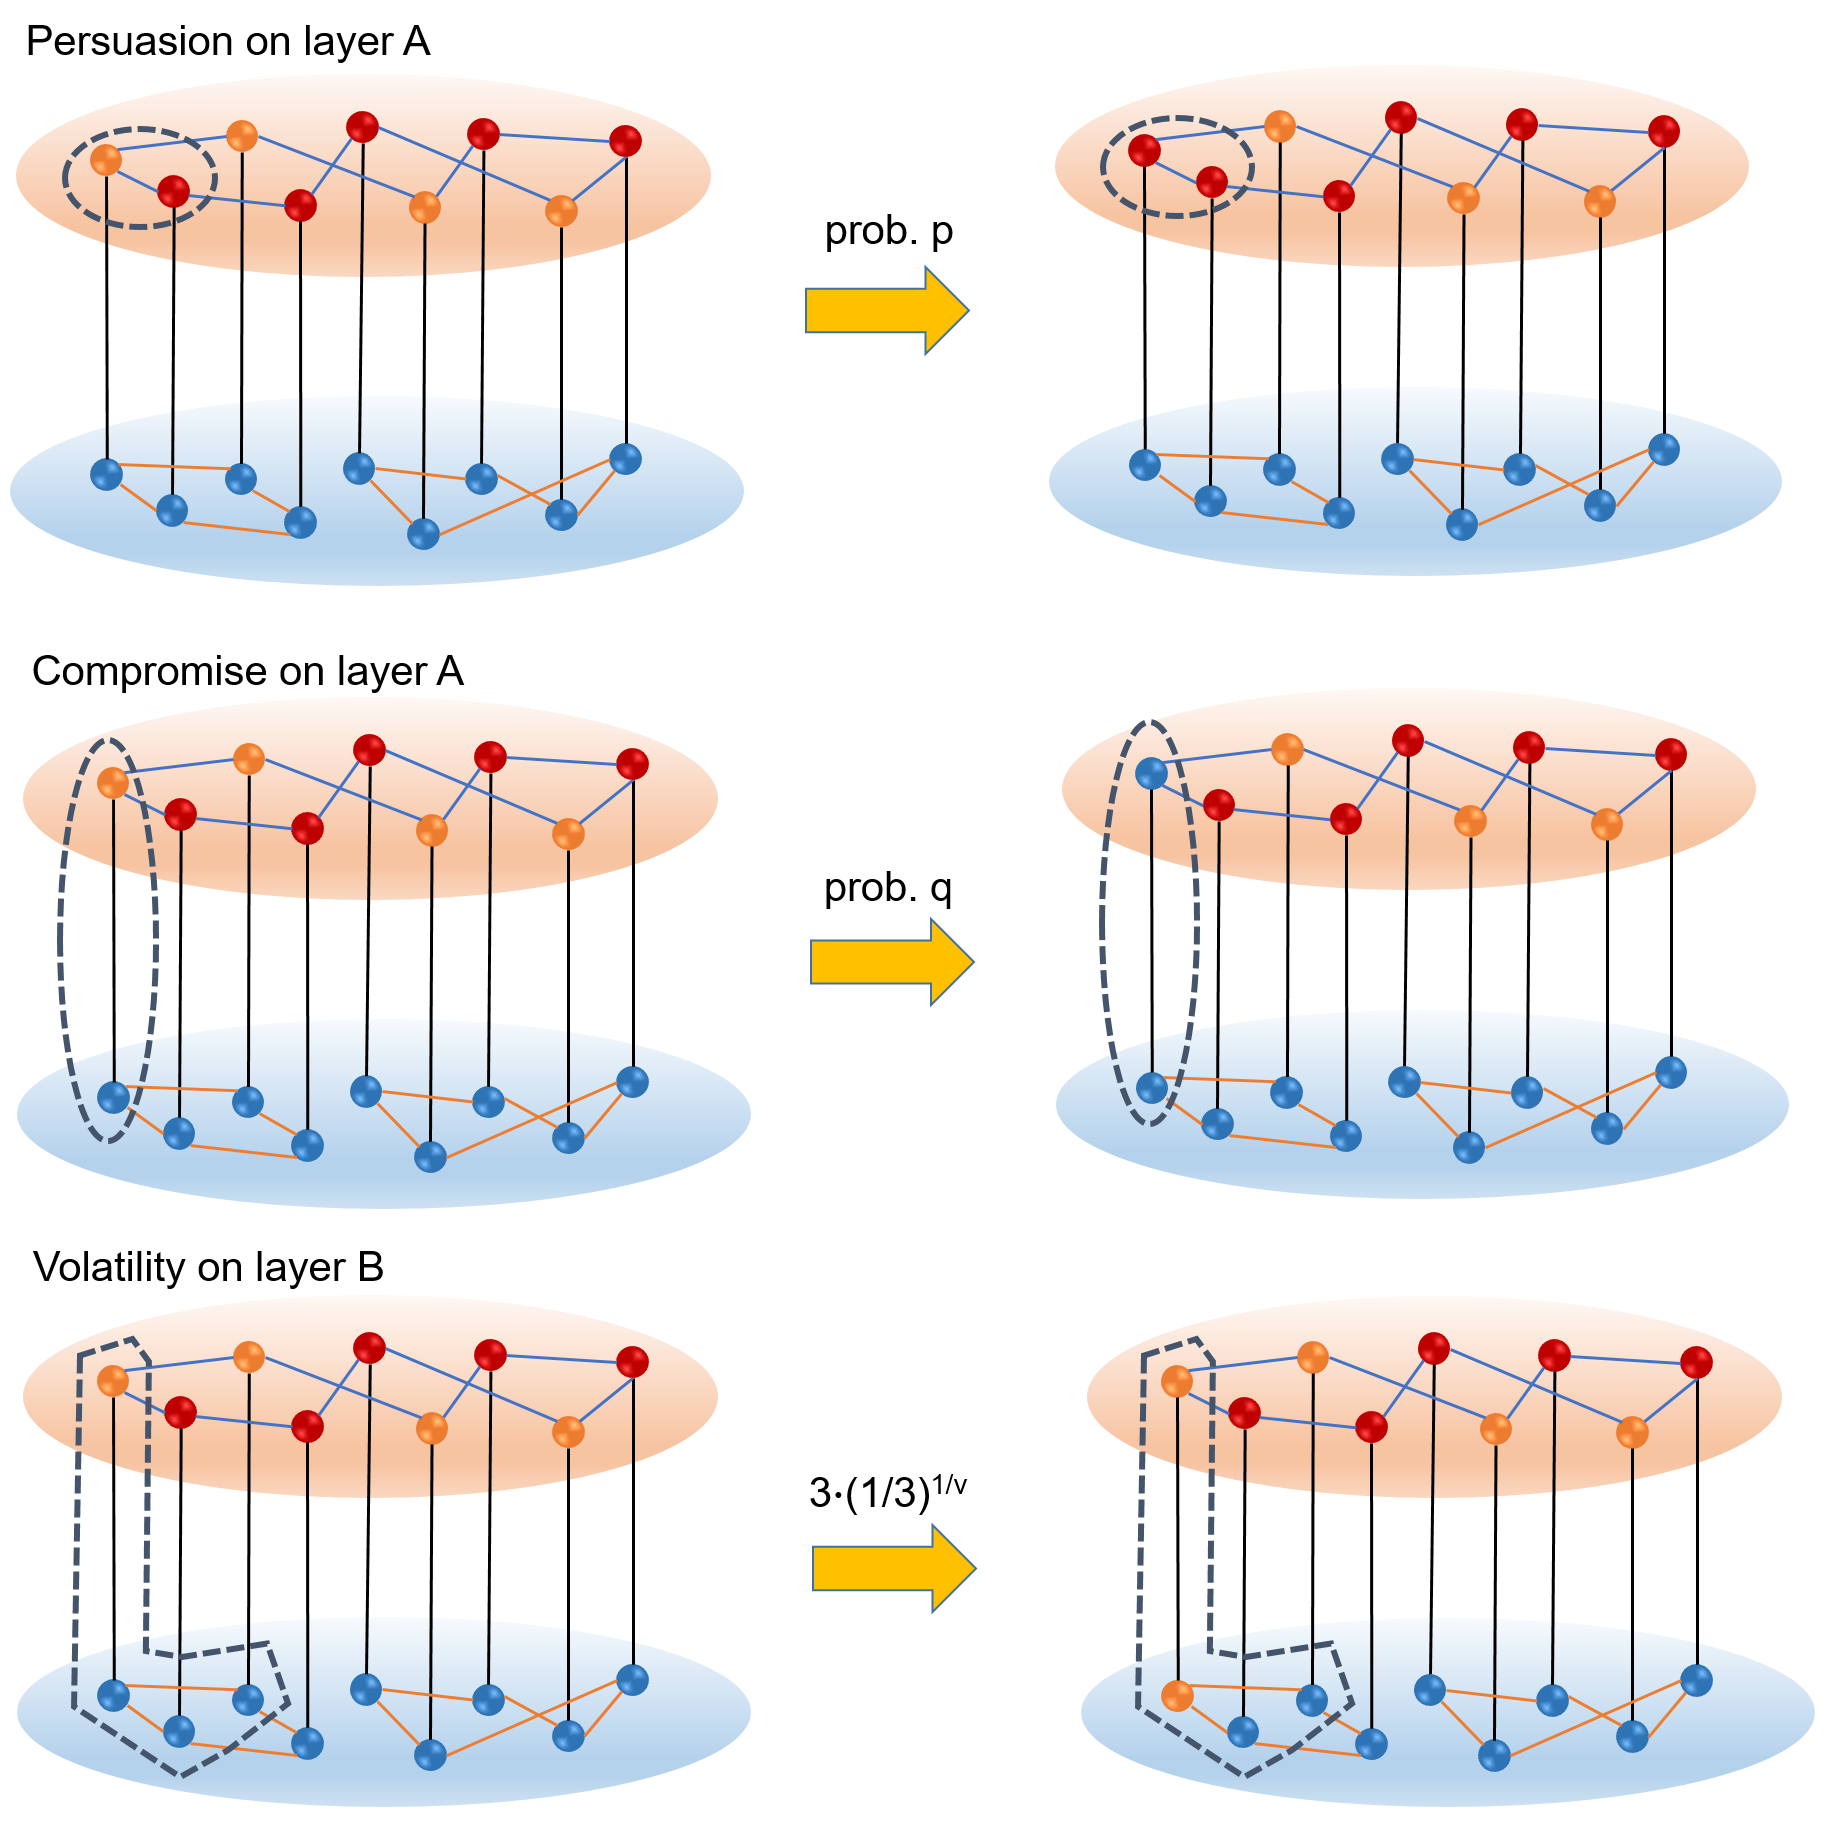
\includegraphics[width=\hsize]{total_dynamics.png}
	\caption{The example of dynamics on two layers}
	\label{total_dynamics}
\end{figure}

Fig.~\ref{total_dynamics} shows that how each dynamics work on each layer. In case of that a node in layer A has connection with a neighbor node in layer A or layer B, if two nodes are same orientation, persuasion dynamics works on this link(but only for nodes in layer A), otherwise two nodes have different orientations each other, compromise dynamics works on this link(but only for nodes in layer A). Dynamics on layer A works considering only links between two nodes. While, a node in layer B is different with a node in layer A. Dynamics on layer B works considering all links connected with a node in layer B. As shown in third figure(Fig.~\ref{total_dynamics}), when a node changes its state, it considers all connected links including internal and external links. According to calculated probability, a node in layer B can change its state or not.    

There are two parameters in the dynamics of layer A. To simply represent the probability $p$ and probability $q$ together, we set $p+q=1$. So, $p$ represents the tendency of opinion such as extreme or moderate, which is scaled to be $0$ to $1$. And, the scale of $v$, in the dynamics of layer B, is also $0$ to $1$. 

\section{Simulations and Analysis}
To start with a polarized competition, as the initial conditions, nodes in layer A are all positive, and nodes in layer B are all negative as shown in Fig.~\ref{competition}. For nodes in layer A, it begins with the status where half of nodes are $+1$ and the others are $+2$. The initial state of nodes in layer B have only $-1$.
 
\begin{figure}[!htb]
	\centering
	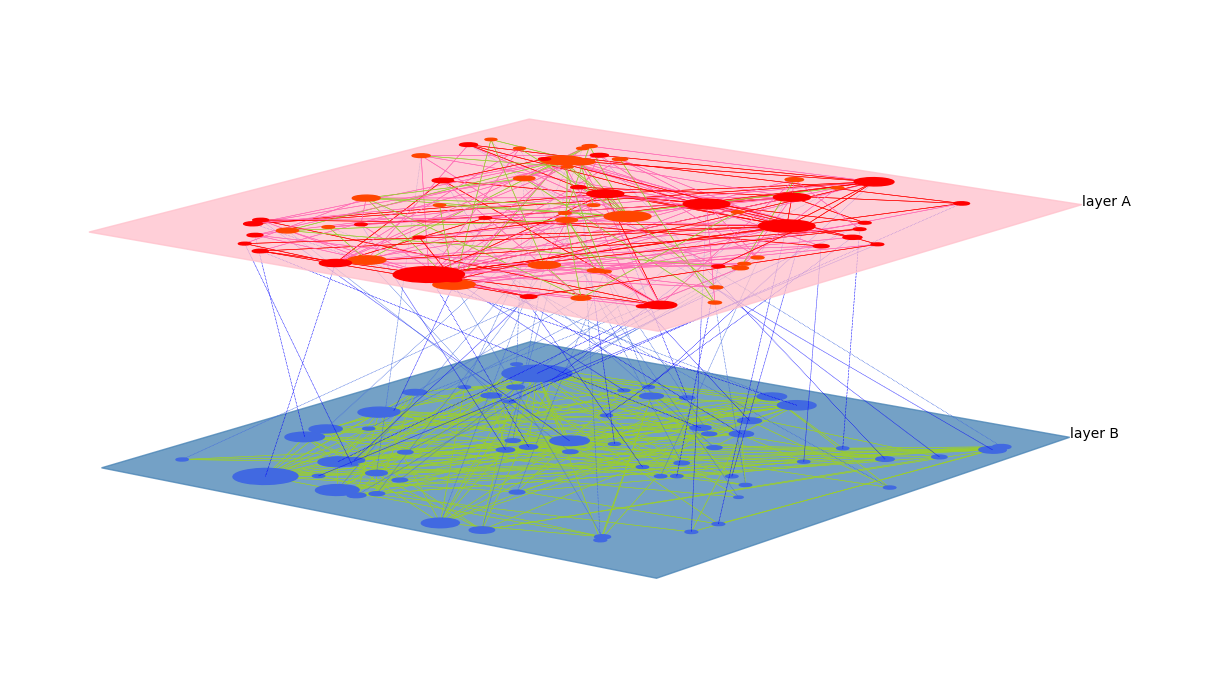
\includegraphics[width=\hsize]{competition.png}
	\caption{Competition of Interconnected Network}
	\label{competition}
\end{figure}

To implement the interconnected dynamics, one step consists of two layers dynamics, where every node in layer A will be checked with opinion dynamics, and every node in layer B will updates its state according to the decision-making dynamics. Here, we would control dynamics orders between layers and updating rules of nodes states. With changing dynamics orders and updating rules, it would be investigated how state of network change.      

Each simulation takes $100$ steps, and $100$ simulations are considered for average results. In the following simulations, we use \textit{`Average State'(AS)} and \textit{`Consensus Index'(CI)} to measure the competition result.

\begin{equation}
AS = avg\left( {\sum\limits_i^{{K^A}} {S_i^A/4} } \right) + avg\left( {\sum\limits_i^{{K^B}} {S_i^B/2} } \right).
\end{equation}

\begin{equation}
CI = \frac{{({K_ + }^A \cdot {K_ - }^B) + ({K_ - }^A \cdot {K_ + }^B)}}{{{K^A} \cdot {K^B}}}
\end{equation}

In these formula, $S_i^A$ means the state of node \textit{i} in layer A, and $K^A$ is the number of nodes in layer A. ${K_ + }^A$ represents the number of nodes with positive state in layer A.   

With \textit{AS}, it could be verified whether the consensus happens in accordance with $p$ and $v$.  If the positive consensus happens, it would be close to the value of $+1$ and if the negative consensus happens, it would be close to the value of $-1$. The values between $+1$ and $-1$ mean the states are belonging to the coexistence part.

With \textit{CI}, it could be measured how close the network state is to consensus. If the \textit{CI} is close to $0$, the state is close to positive or negative consensus. If the \textit{CI} is close to $1$, the state is separated coexistence where states of all nodes in layer A is opposed to states of all nodes in layer B. If the \textit{CI} is close to $0.5$, the state is mixed coexistence where each layer has both positive and negative states of nodes.    

\subsection{Competition on two-layer Networks}
\label{competition on two-layer networks}
Prior to comparing with updating rules, we try to understand competition on two-layer networks. To comprehend the competition of two layers, simulation results would be analyzed with several indexes and figures described in ~\ref{modeling}. Here, both dynamics orders between layers and updating rules of nodes states follow the sequential orders. Dynamics order between layer follows that layer B is updated after layer A is updated. Updating rule of nodes follows each node is sequentially updated considering all connected links individually. 
 
The simulation results are shown in Fig.~\ref{AS_2d} and Fig.~\ref{p_v_AS_3d}. Fig.~\ref{AS_2d}(a) shows that when $p > 0.2$, $0.37 < v < 0.47$, it normally tends to positive consensus. But, if $v$ is lower or larger than certain values, it doesn't make consensus.
In Fig.~\ref{AS_2d}(b), as $v$ increases, the state of networks changes continuously. But, when $p$ is very low($p \le 0.05$), it doesn't make positive consensus. On the other hands, when $p$ is large enough, it has the most positive consensus parts. When $v$ are large enough($>0.6$) and less than $1$, the state is in a coexistence part.

\begin{figure*}[!htb]
	\centering
	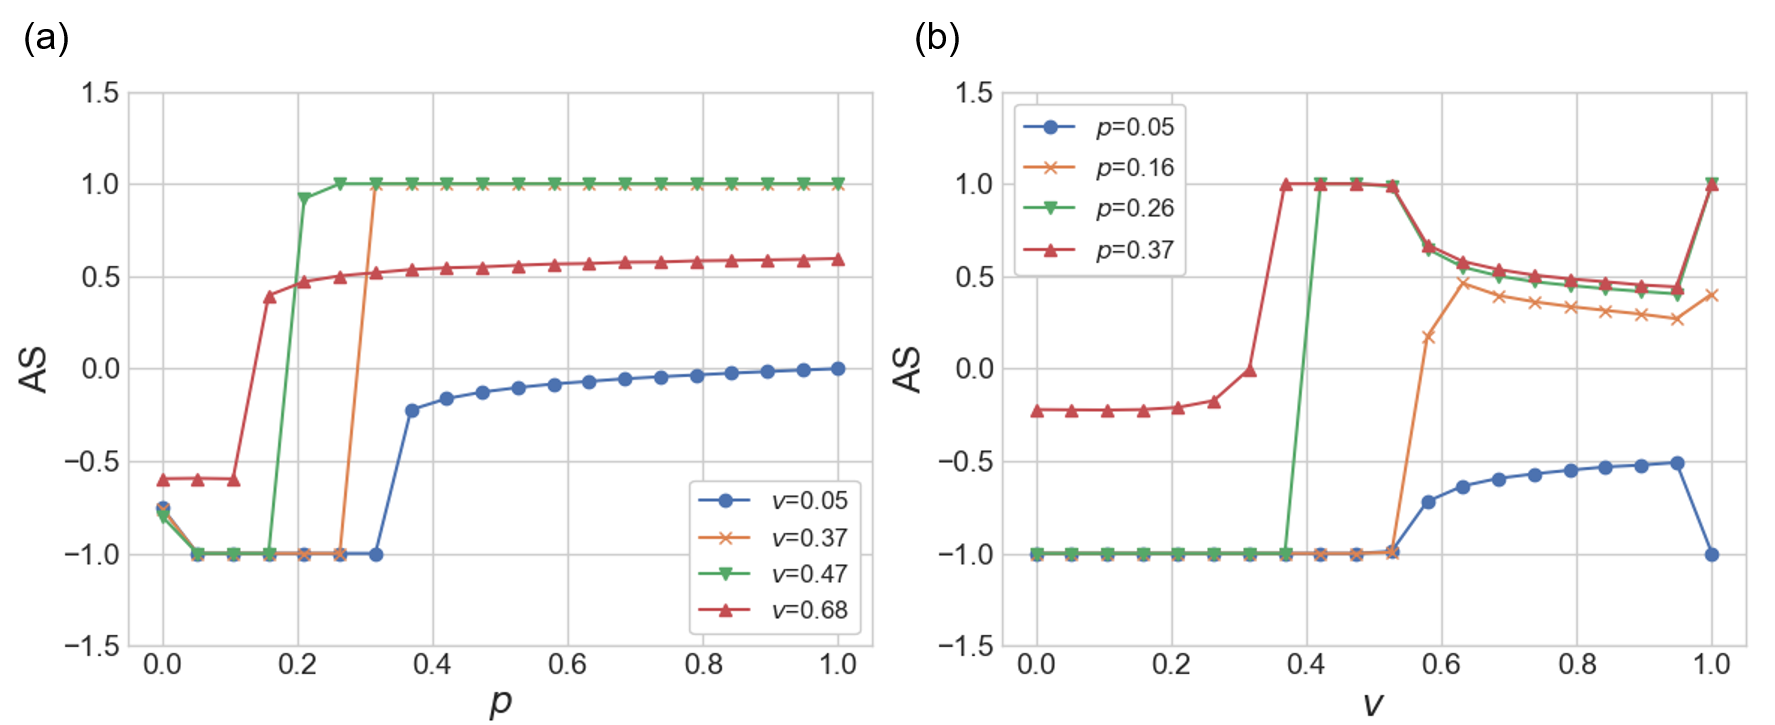
\includegraphics[width=\hsize]{AS_2d.png}
	\caption{(a) $p$-\textit{AS} chart according to certain $v$ values. (b) $v$-\textit{AS} chart according to certain $p$ values.}
	\label{AS_2d}
\end{figure*}

\begin{figure}[!htb]
	\centering
	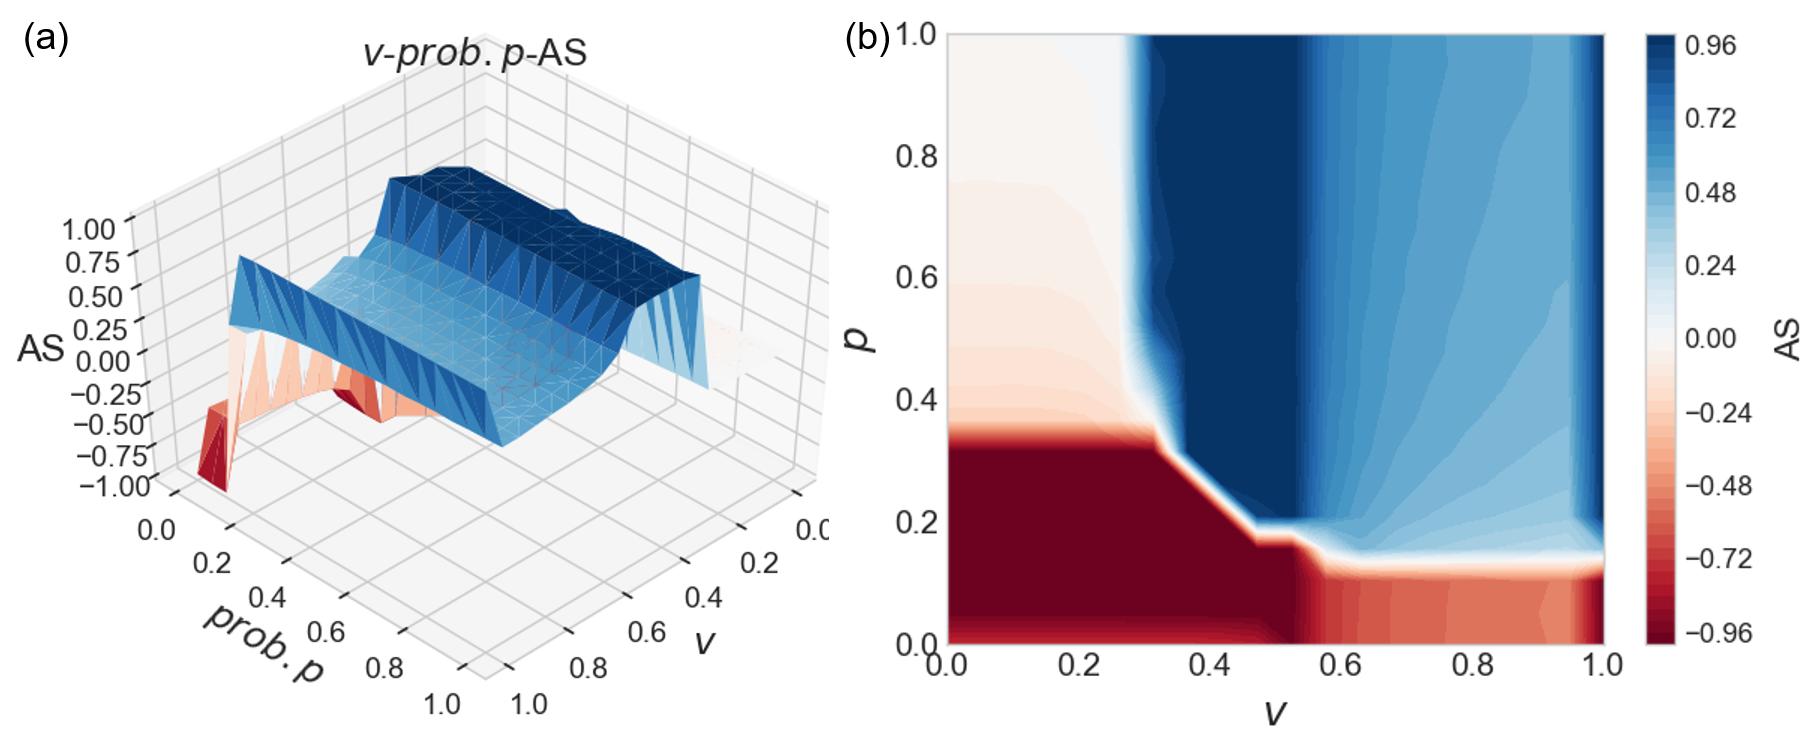
\includegraphics[width=\hsize]{p_v_AS_3d.png}
	\caption{Two layer networks with sequential updating rule : \textit{AS} changing with all $p$ and $v$}
	\label{p_v_AS_3d}
\end{figure}


Fig.~\ref{p_v_AS_3d} shows the states of two layers according to all $p$s and all $v$s. The $X$-axis is the $p$ and the $Y$-axis is the $v$, and the $Z$-axis represents \textit{AS}. The closer the color is to blue, the more it has positive consensus. And the closer the color is to red, the more it has negative consensus. A light and white areas have coexistence with positive states and negative states. This chart has two areas for coexistence, when $v$ is very low or very high. When $v$ is in certain range, interconnected network can perform positive or negative consensus with different $p$ values. 

\begin{figure}[!htb]
	\centering
	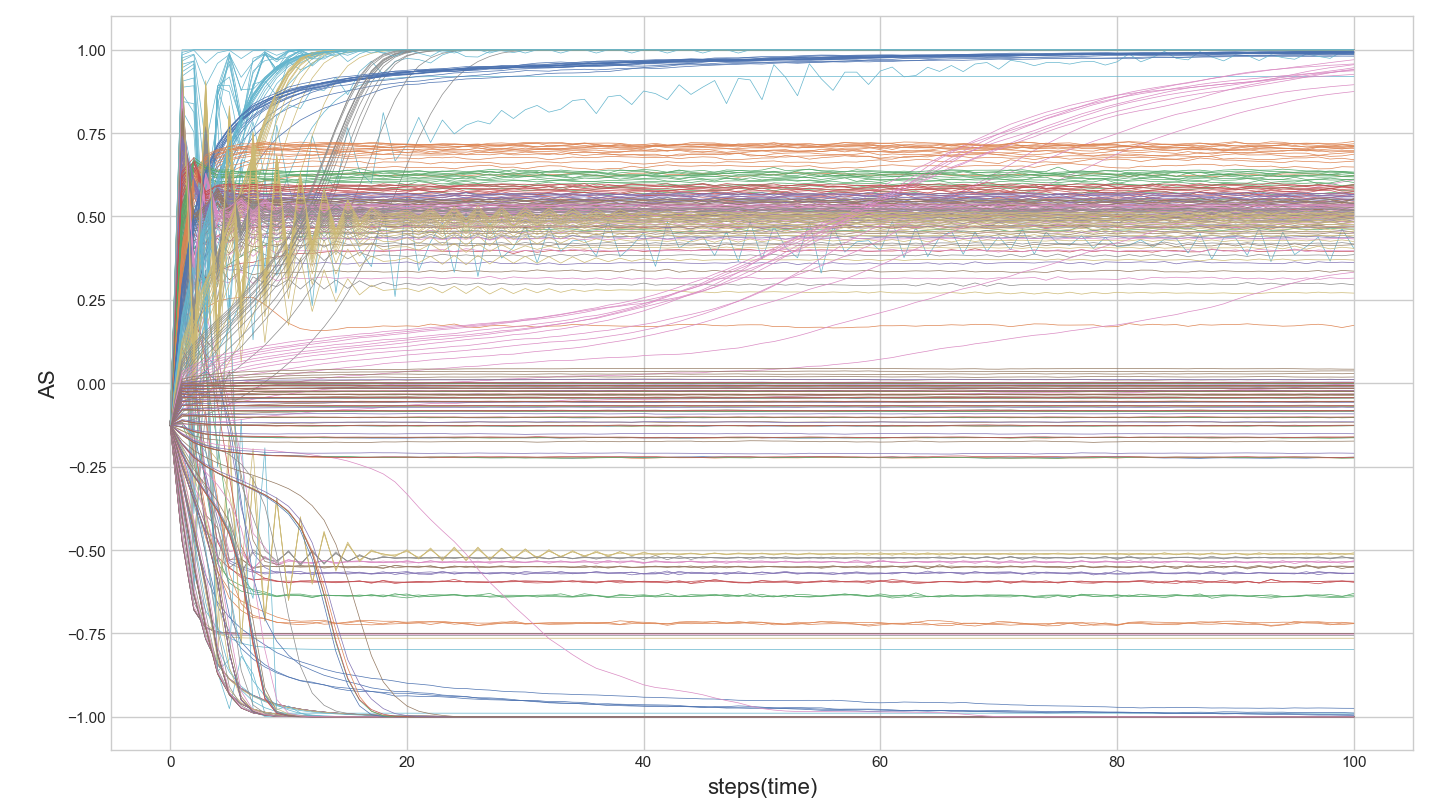
\includegraphics[width=\hsize]{timeflow_AS.png}
	\caption{Two layer networks with sequential updating rule : \textit{steps-AS} changing with all $p$ and $v$}
	\label{timeflow_AS}
\end{figure}

Fig.~\ref{timeflow_AS} shows \textit{AS} value according to each step(time). As the steps are increased, the states of two-layers become stable. The closer \textit{AS} value is to $+1$, the closer the state is to positive consensus. The closer \textit{AS} value is to $-1$, the closer the state is to negative consensus. \textit{AS} values between $+1$ and $-1$ represents coexistence states, but it cannot be classified whether they are mixed coexistence states or separated coexistence states.
\begin{figure}[!htb]
	\centering
	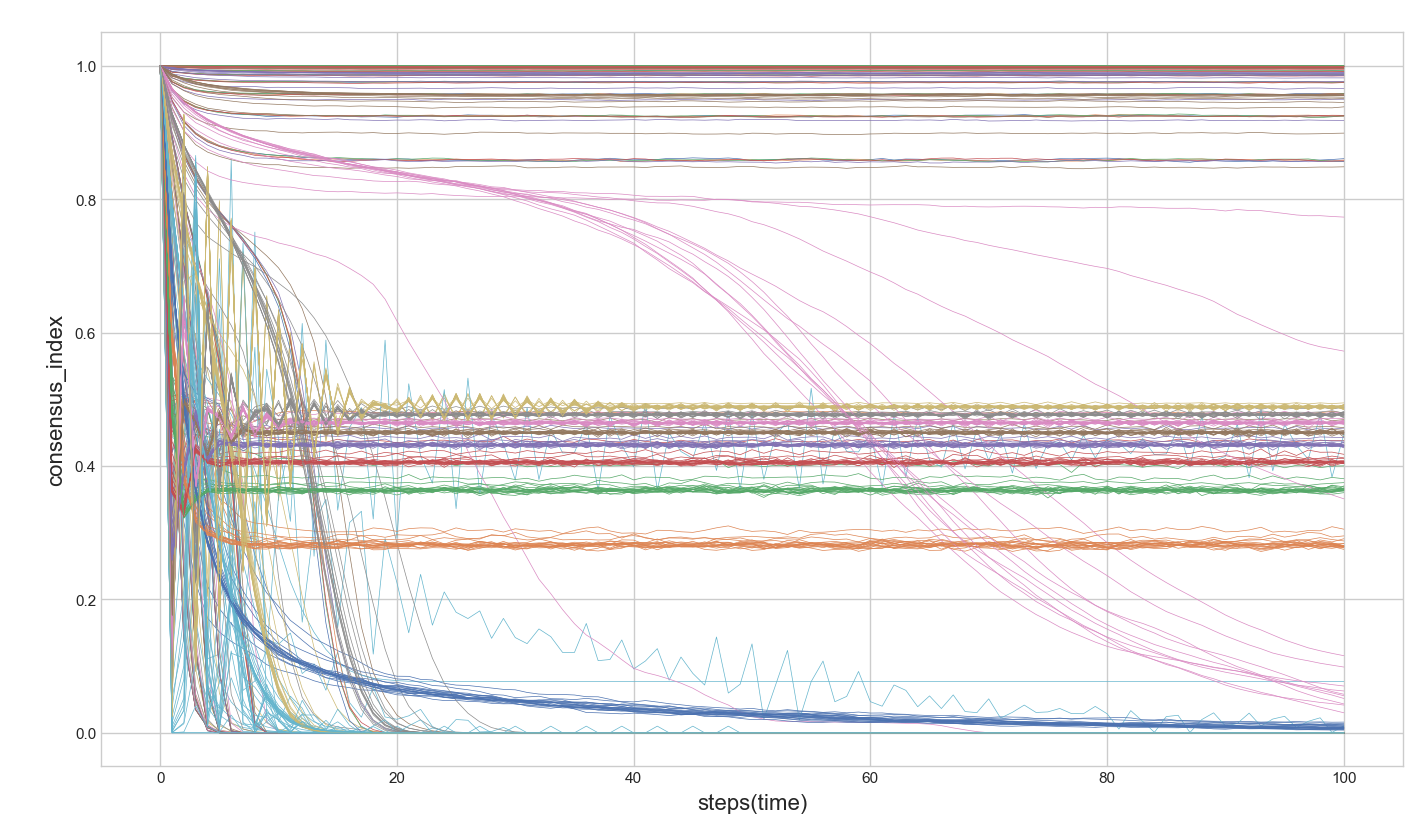
\includegraphics[width=\hsize]{timeflow_CI.png}
	\caption{Two layer networks with sequential updating rule :\textit{steps-CI} changing with all $p$ and $v$}
	\label{timeflow_CI}
\end{figure}
Fig.~\ref{timeflow_CI} shows \textit{CI} value according to each step(time). With \textit{CI}, the coexistence states of two-layer can be classified into mixed coexistence states and separated coexistence states. Mixed coexistence states mean that each layer has both positive and negative states, and separated coexistence states indicate that each layer has only one state, but a layer is opposite to the other layer. As the \textit{CI} value is close to $0.5$, the states are close to mixed coexistence states. And, as the \textit{CI} value is close to $1$, the states are close to separated coexistence states. If the values are close to $0$, the states are close to consensus states.(Here, it is impossible to divide whether they are positive consensus or negative consensus.)           

Here, with the indexes(\textit{AS}, \textit{CI}), simulation results can be categorized whether they are convergent to consensus or coexistence. It is found out that there exists 3 parts(positive consensus, negative consensus, coexistence) on competitions between two layers according to parameters. And, as known in fig.~\ref{timeflow_AS} and fig.~\ref{timeflow_CI}, the state of networks becomes stable as time goes by. Next simulations would also use these indexes for categorizing the results. 

\subsection{Simulations with various updating rules}
When considering dynamics orders and updating rules on two-layer networks, there are many ways to update the state of nodes. Dynamics order of two layer can be considered whether layer A works first or layer B. And, nodes can be thought about whether the states of nodes are changed simultaneously or sequentially or randomly. Links connected with a node also can be deliberated whether links are activated on a node sequentially or simultaneously or randomly. But, in layer B dynamics, order of links in one node is always for simultaneous updating rule, because dynamics formula of layer B already considers states of all connected neighbor nodes simultaneously. To sum up, as shown in Table.\ref{table1}, 25 updating rules would be considered according to layers, nodes, and links. 
\begin{table}[htp]
	\scriptsize
	\begin{center}
		\begin{tabular}{c|c|c|c|c}
			Order of layers                                  & \multicolumn{2}{|c|}{Layer A}                                      & Layer B                & remarks   \\ \cline{2-4}
			& Order of nodes                 & Order of links                     & Order of nodes         &  \\ \hline
			\multirow{10}{*}{Layer A $\rightarrow$ Layer B} & \multirow{4}{*}{Sequential}    & \multirow{2}{*}{Sequential}        & Sequential             & O(o, o) $\to$ D(o) \\  \cline{4-5}  
			&                                &                                    & Simultaneous           & O(o, o) $\to$ D(s) \\  \cline{3-5}     
			&                                & \multirow{2}{*}{Simultaneous}      & Sequential             & O(o, s) $\to$ D(o) \\  \cline{4-5} 
			&                                &                                    & Simultaneous           & O(o, s) $\to$ D(s) \\  \cline{2-5} 
			& \multirow{4}{*}{Simultaneous}  & \multirow{2}{*}{Sequential}        & Sequential             & O(s, o) $\to$ D(o) \\  \cline{4-5}
			&                                &                                    & Simultaneous           & O(s, o) $\to$ D(s) \\  \cline{3-5}
			&                                & \multirow{2}{*}{Simultaneous}      & Sequential             & O(s, s) $\to$ D(o) \\  \cline{4-5}
			&                                &                                    & Simultaneous           & O(s, s) $\to$ D(s) \\  \cline{2-5}
			& \multirow{2}{*}{Random}        & \multirow{2}{*}{Random}            & Sequential             & O(r, r) $\to$ D(o) \\  \cline{4-5}
			&                                &                                    & Simultaneous           & O(r, r) $\to$ D(s) \\   \hline
			\multirow{10}{*}{Layer A $\leftarrow$ Layer B}  & \multirow{4}{*}{Sequential}    & \multirow{2}{*}{Sequential}        & Sequential             & O(o, o) $\leftarrow$ D(o) \\  \cline{4-5}  
			&                                &                                    & Simultaneous           & O(o, o) $\leftarrow$ D(s) \\  \cline{3-5}     
			&                                & \multirow{2}{*}{Simultaneous}      & Sequential             & O(o, s) $\leftarrow$ D(o) \\  \cline{4-5} 
			&                                &                                    & Simultaneous           & O(o, s) $\leftarrow$ D(s) \\  \cline{2-5} 
			& \multirow{4}{*}{Simultaneous}  & \multirow{2}{*}{Sequential}        & Sequential             & O(s, o) $\leftarrow$ D(o) \\  \cline{4-5}
			&                                &                                    & Simultaneous           & O(s, o) $\leftarrow$ D(s) \\  \cline{3-5}
			&                                & \multirow{2}{*}{Simultaneous}      & Sequential             & O(s, s) $\leftarrow$ D(o) \\  \cline{4-5}
			&                                &                                    & Simultaneous           & O(s, s) $\leftarrow$ D(s) \\  \cline{2-5}
			& \multirow{2}{*}{Random}        & \multirow{2}{*}{Random}            & Sequential             & O(r, r) $\leftarrow$ D(o) \\  \cline{4-5}
			&                                &                                    & Simultaneous           & O(r, r) $\leftarrow$ D(s) \\   \hline
			\multirow{2}{*}{Layer A $\leftrightarrow$ Layer B}& \multirow{2}{*}{Simultaneous}& Sequential                         & Simultaneous           & O(s, o) $\leftrightarrow$ D(s) \\ \cline{3-5}
			&                                & Simultaneous                       & Simultaneous           & O(s, s) $\leftrightarrow$ D(s) \\ \hline
			\multirow{3}{*}{Layer A $\Leftrightarrow$ Layer B}& \multirow{2}{*}{Sequential}  & Sequential                         & Sequential             & O(o, o) $\Leftrightarrow$ D(o) \\ \cline{3-5}
			&                                & Simultaneous                       & Sequential             & O(o, s) $\Leftrightarrow$ D(o) \\ \cline{2-5}
			& Random                         & Random                             & Random                 & O(r, r) $\Leftrightarrow$ D(r) \\ \hline
			
		\end{tabular}
	\end{center}
	\caption{25 updating rules according to order of layers, nodes and links}
	\label{table1}
\end{table}

In Table.~\ref{table1} remarks, 'O(o, o) $\to$ D(s)’ means Opinion layer(node : sequential order updating, edges : sequential order updating) $\to$ Decision Making layer(node : simultaneous updating). And 'O(o, o) $\Leftrightarrow$ D(o)’ means that one node in opinion layer is updated, and then one node in decision making layer is updated, this rule is repeated until all nodes are updated. Dynamics with 25 updating rules are simulated with parameter $p=0.4$ and $v=0.4$. Simulation results are analyzed according to layers, nodes and link. 
 
\subsubsection{Order of layers}
There exist two layers on interconnected network. And each layer has its own dynamics, such as \textit{M-Model} dynamics and \textit{AS-Model} dynamics. Two dynamics can be operated simultaneously or sequentially. If they act sequentially, dynamics of layer A can act first or dynamics of layer B can work previously. Otherwise, regardless of layers order, nodes of two layers can interact mutually. For example, one node in layer A are updated and then one node in layer B are updated until all nodes are updated.  
Considering all situations, there are 4 ways in order of two layers, \textit{Layer A $\to$ Layer B, Layer A $\leftarrow$ Layer B, Layer A $\leftrightarrow$ Layer B(simultaneous), Layer A $\Leftrightarrow$ Layer B(interaction regardless of layers)}. 
\begin{figure}[!htb]
	\centering
	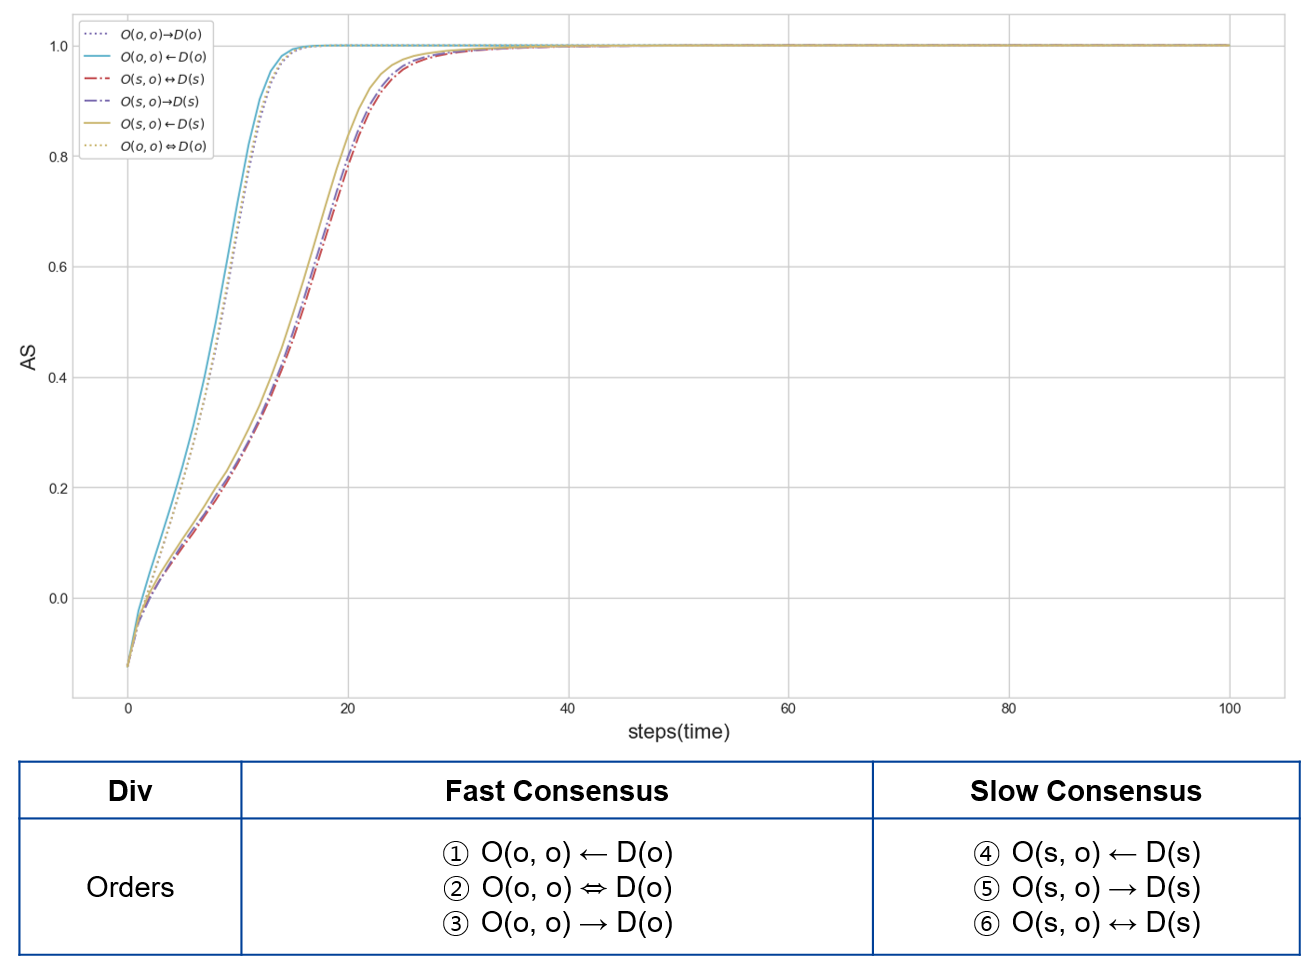
\includegraphics[width=\hsize]{layerorder.png}
	\caption{Simulation results according to layer orders}
	\label{layerorder}
\end{figure}
As seen in Fig.~\ref{layerorder}, simulation results show that there is little difference between orders of layers. Consensus time and result are almost same, though dynamics order is different. Regardless of dynamics directions, when other conditions, such as order of nodes and edges are same, the dynamics results are also very similar.  

\subsubsection{Order of nodes}
In the simulation model, each layer has $2048$ nodes, and each node has interaction with other nodes. Now, interaction order of nodes would be considered. One node can be updated after other nodes are updated sequentially. Otherwise, every node can be updated simultaneously. Simulation results would be different according to interaction order of nodes. In addition, random order between nodes is also simulated. In random order, one link is selected randomly and updated regardless of orders between nodes and links until all links are considered. Interaction order of nodes is related to time. If networks have short time to change states, networks follow simultaneous updating rule. However, if networks have enough time to update states, networks follow sequential updating rules. In real world, discussion or conversation with enough time indicates sequential updating rule of nodes, and voter or election means simultaneous updating rule of nodes. 

\begin{figure}[!htb]
	\centering
	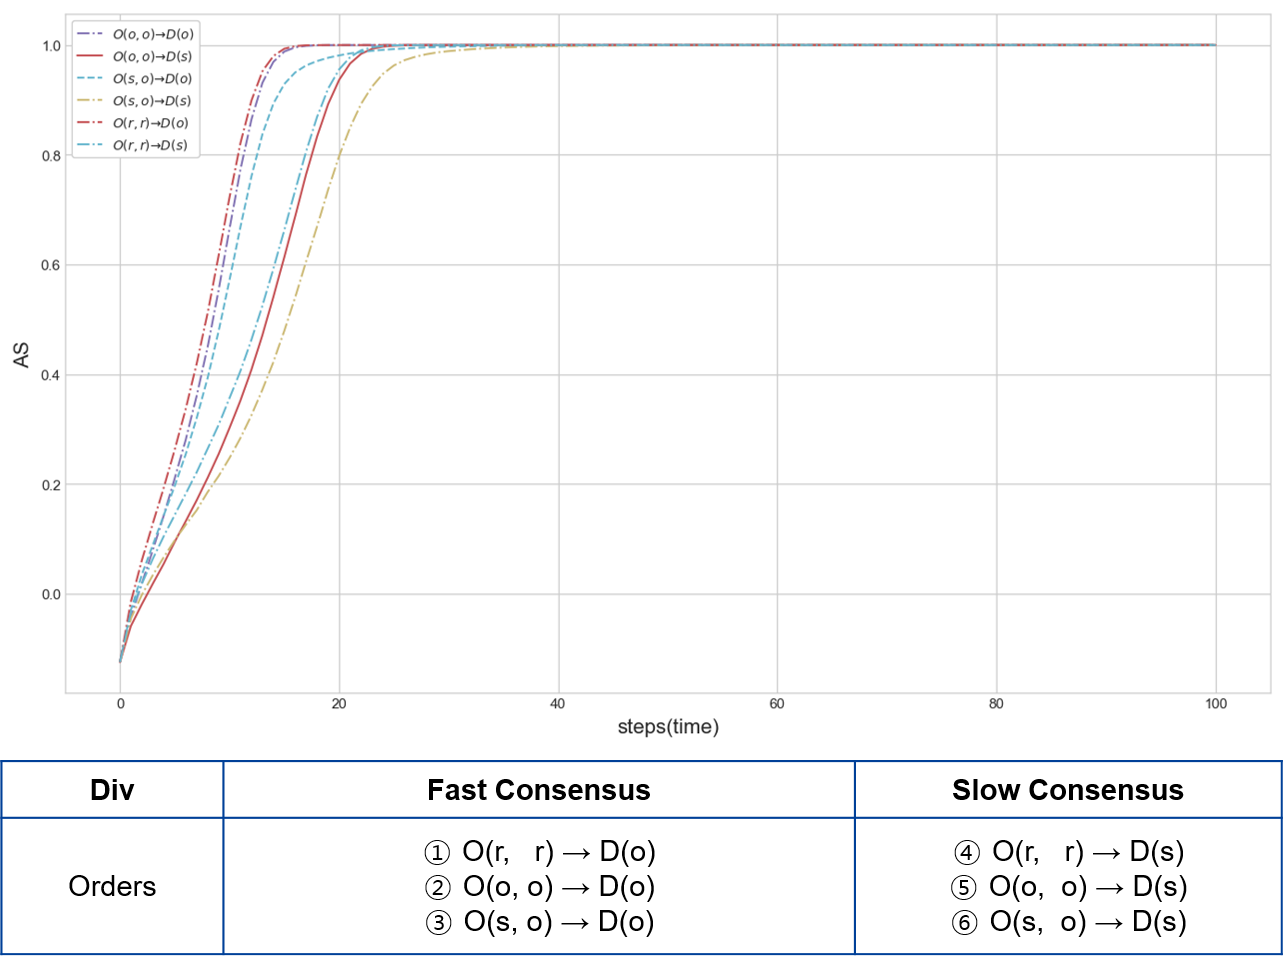
\includegraphics[width=\hsize]{nodeorder.png}
	\caption{Simulation results according to node orders : comparison between order of nodes under same conditions}
	\label{nodeorder}
\end{figure}
Fig.~\ref{nodeorder} shows simulation results. The results are classified to two categories, fast consensus and slow consensus. And it shows that simultaneous interaction between nodes makes slow consensus. Simultaneous order in layer A does not make large difference, but it make consensus slightly slow. Simultaneous interaction between nodes in layer B have more influence on consensus time than in layer A. Random order has similar results with sequential order and does not make different states. For quick social consensus, both opinion layer and decision making layer need sequential updating rule, such as conversation and discussion.      

\subsubsection{Order of links}
Each node has several links connected with other nodes. Simulation results can be different according to that links are operated sequentially or simultaneously. If links of each node work sequentially, a state of node is changed whenever each link is activated. However, If link of a node work simultaneously, a state of node would be changed considering all connected nodes. In real world, order of links in one node can be analyzed as characteristics of nodes. If order of links is sequential, the node would be rash. If order of links is simultaneous, the node would be considerate. 
\begin{figure}[!htb]
	\centering
	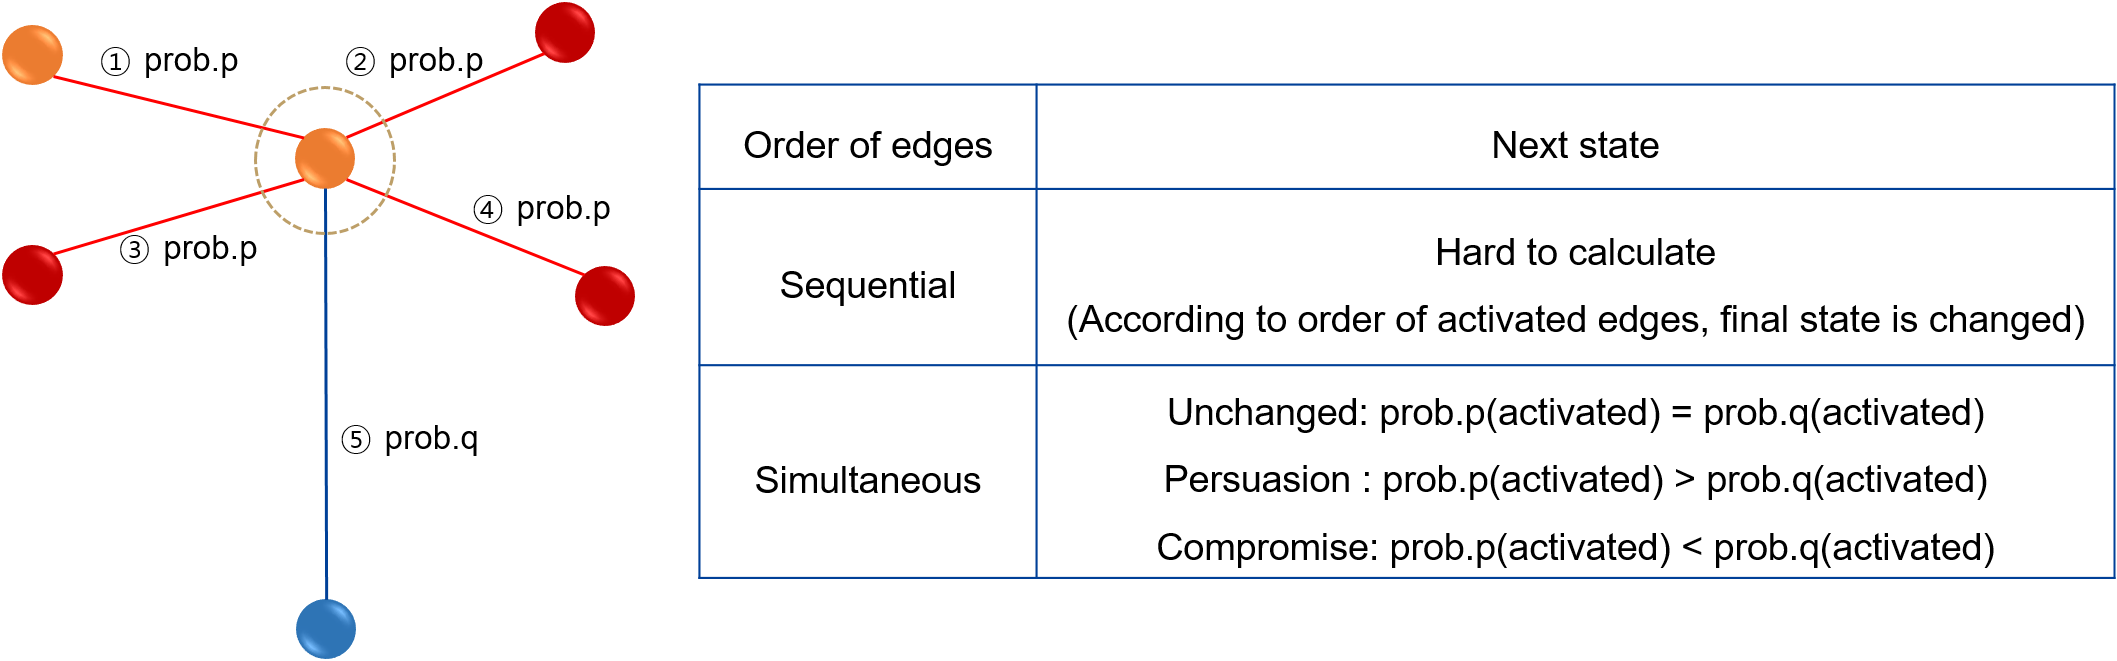
\includegraphics[width=\hsize]{edgeorder_explanation.png}
	\caption{one node connected with other nodes changes its state with sequential or simultaneous order of edges}
	\label{edgeorder_explanation}
\end{figure}  
For example, considering the case that one node is connected with other nodes as shown in Fig.~\ref{edgeorder_explanation}, we can think how the state of node changes. 
If the links follow sequential updating rule, it is hard to calculate the probabilities, because the states can change according to sequential order of links. Therefore, we can get next states of nodes by using computer simulation 

If the links follow simultaneous updating rule, it needs some assumptions for calculation: 
\begin{enumerate}[(1)]
	\item If the number of activated \textit{prob.p} is more than the number of activated \textit{prob.q}, persuasion dynamics would work. 
	\item If the number of activated \textit{prob.p} is same with the number of activated \textit{prob.q}, the state would be unchanged.
	\item If the number of activated \textit{prob.p} is less than the number of activated \textit{prob.q}, compromise dynamics would work.
\end{enumerate}

Through these assumptions, we can calculate probabilities of changing state in layer by considering all cases like these formula.  

\begin{equation}
\begin{array}{l}
K = \{ k \quad|\quad 0, \cdots ,{n^{ - {S_i}}}\}, \quad L = \{l \quad|\quad 0, \cdots ,{n^{{S_i}}}\},
\quad M = \{m \quad|\quad k-l\}, \\
{P_A}({S_i} \mapsto {{S'}_i}) = \begin{cases}
\mbox{unchanged}(k = l):\sum {{p^{{n^{ - {S_i}}}+m}} \cdot {{(1 - p)}^{{n^{{S_i}}}-m}} \cdot {}_{{n^{{S_{^i}}}}}{C_k} \cdot {}_{{n^{ - {S_{^i}}}}}{C_l}} \\
\mbox{persuasion}(k > l):\sum {{p^{{n^{ - {S_i}}}+m}} \cdot {{(1 - p)}^{{n^{{S_i}}}-m}} \cdot {}_{{n^{{S_{^i}}}}}{C_k} \cdot {}_{{n^{ - {S_{^i}}}}}{C_l}} \\
\mbox{compromise}(k < l):\sum {{p^{{n^{ - {S_i}}}+m}} \cdot {{(1 - p)}^{{n^{{S_i}}}-m}} \cdot {}_{{n^{{S_{^i}}}}}{C_k} \cdot {}_{{n^{ - {S_{^i}}}}}{C_l}} 
\end{cases}
\end{array}
\end{equation}

\begin{figure}[!htb]
	\centering
	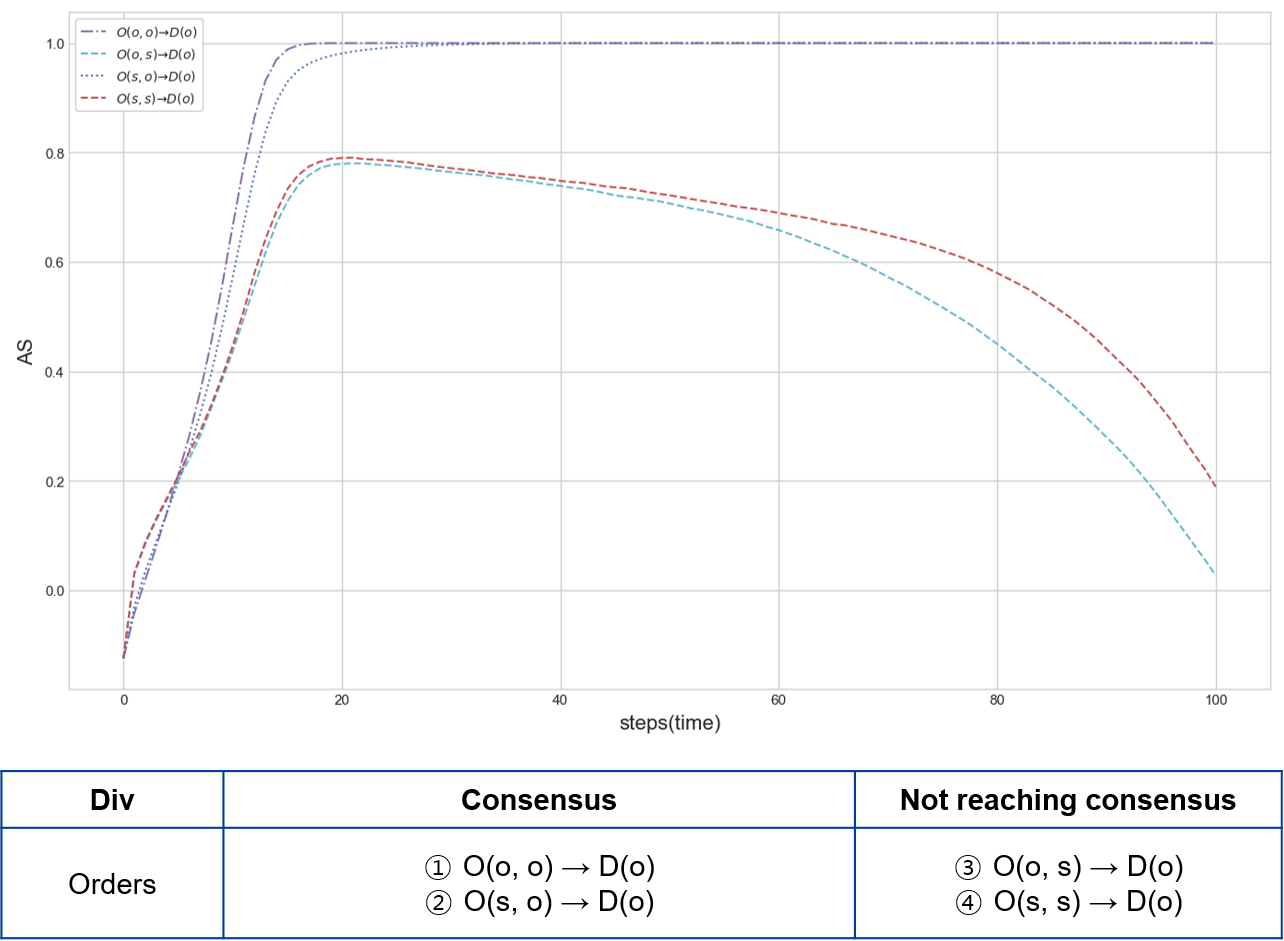
\includegraphics[width=\hsize]{edgeorder.png}
	\caption{Simulation results according to link orders : comparison between order of edges under same conditions}
	\label{edgeorder}
\end{figure}
Fig.~\ref{edgeorder} shows the simulation result according to order of links. The results are categorized to consensus and coexistence(not reaching consensus) due to order of links.
Sequential updating rule of links makes consensus, i.e. rash nodes make consensus. But simultaneous updating rule of links makes it hard to reach consensus, i.e. considerate nodes do not make consensus. It can be analyzed that rash node is easy to be extreme and make consensus, but considerate node is very moderate and hard to reach consensus. 

\subsection{Comparison and Analysis}
Comparing with various updating rules on competition between two layers, it would be found out that there are different simulation results according to orders of layers, nodes, and links. To sum up all updating rules, they can be categorized into 3 parts, positive consensus, coexistence, and negative consensus as shown in Fig.~\ref{ordertotal}.  
\begin{figure}[!htb]
	\centering
	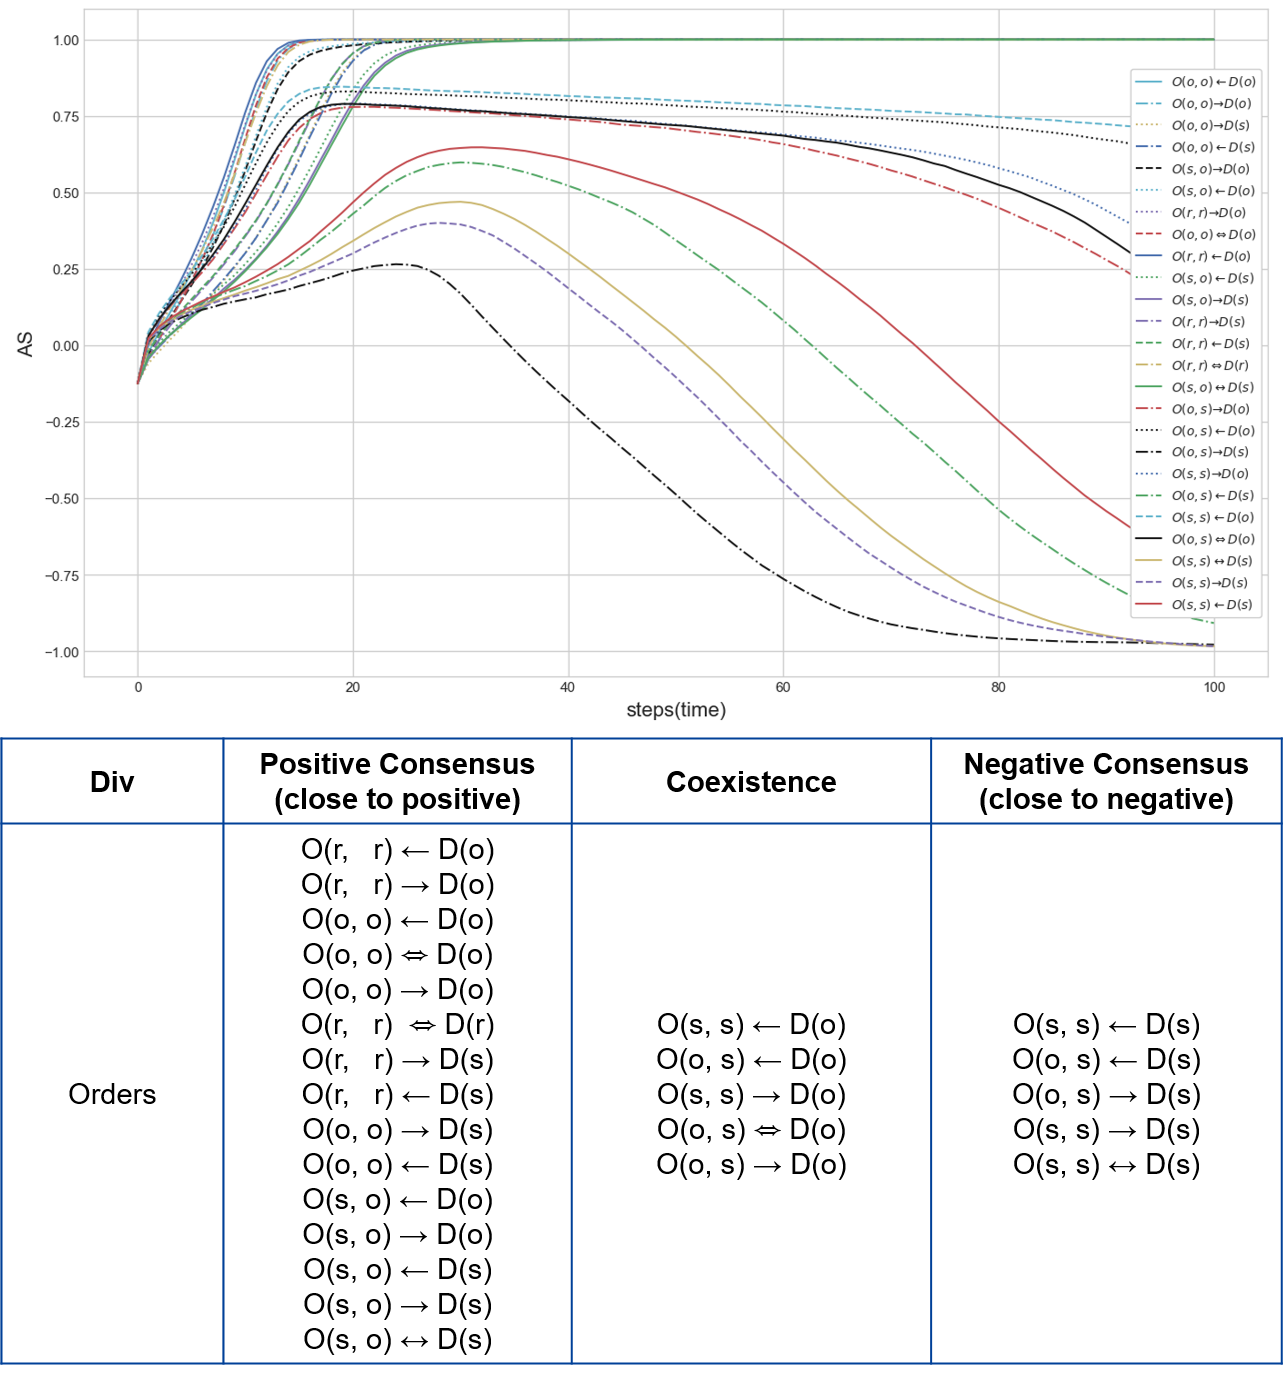
\includegraphics[width=\hsize]{ordertotal.png}
	\caption{Total results of 25 updating rules with \textit{AS}}
	\label{ordertotal}
\end{figure}

To clearly classify the state of two-layers, the results can be analyzed by using \textit{CI} as shown in Fig.~\ref{ordertotal2}. There are three branch points. In the first branch point, the results are divided according to whether order of nodes in layer B is sequential or simultaneous. In the second and third branch point, the results are classified according to whether order of edges in layer A is sequential or simultaneous. As the results, there are 4 categories such as fast positive consensus, slow positive consensus, coexistence and slow negative consensus.
 
\begin{figure}[!htb]
	\centering
	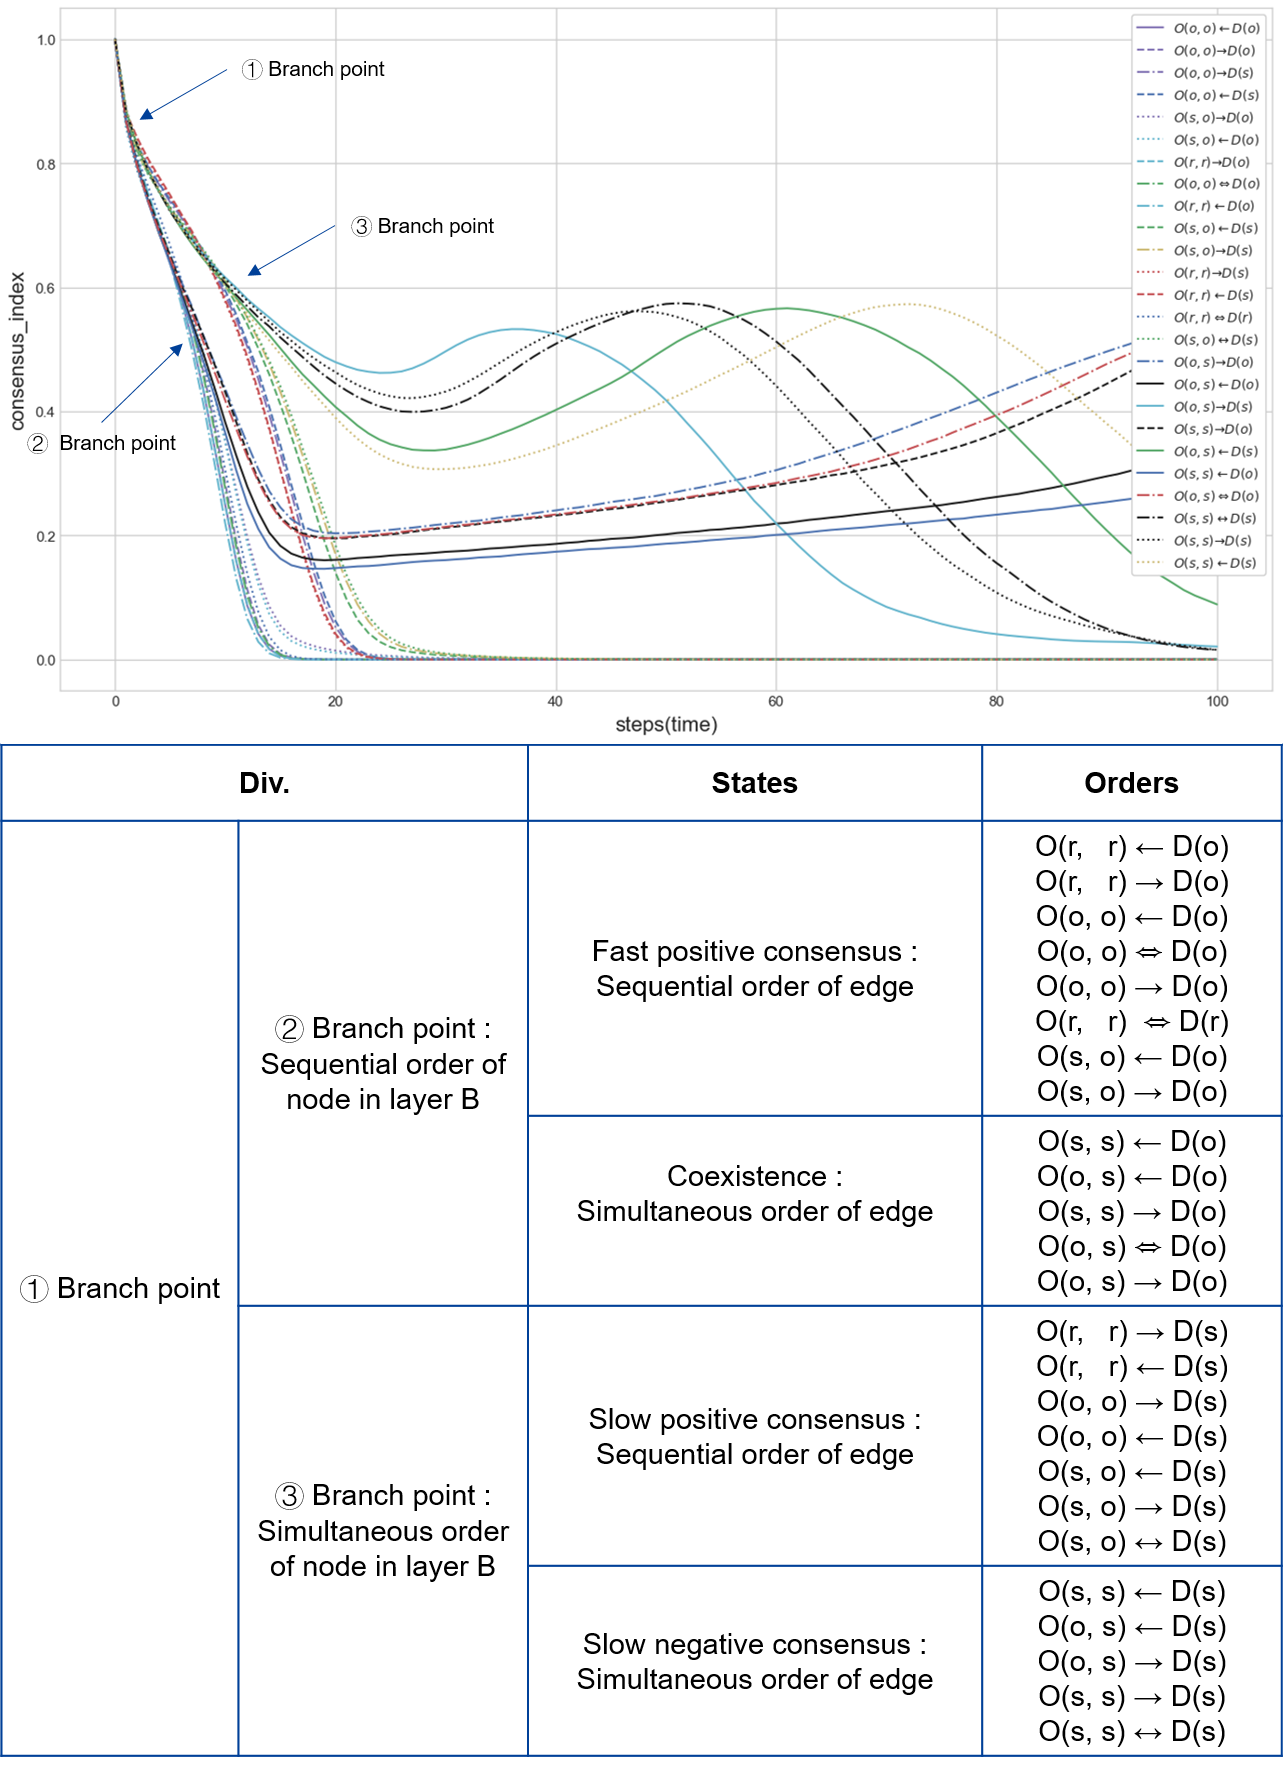
\includegraphics[width=\hsize]{ordertotal2.png}
	\caption{Total results of 25 updating rules with \textit{CI}}
	\label{ordertotal2}
\end{figure}

Through the simulation results, several important facts can be arranged. First, networks with more simultaneous updating rules make slow consensus or coexistence, sometimes make transition to opposite orientation. On the other hands, networks with more sequential updating rules make fast consensus. In other words, if opinion layer has more rash nodes and more time to have conversation and decision making layer has more time to discuss topics, the network have more probabilities to make consensus for state of opinion layer. Second, dynamics order between layers does not have an influence for network state, though there exists tiny consensus time gap. Third, order of nodes in layer B has more influence for network states than order of nodes in layer A. order of nodes in layer B makes the first branch point. But order of nodes in layer A does not make any branch point, though there exists tiny consensus time gap. Forth, order of links in layer A is strongly influential so that it makes different network states, i.e. characteristics of nodes in layer A, such as rash and considerate, affects consensus time and sometimes makes transition to coexistence or opposite orientation. 


\section{Conclusion}
In this work, we have researched competition on interconnected networks, where layer A is a layer of social opinion and layer B is a network representing decision making.  Especially, we have focused on dynamics order and updating rules on competition between two layers. When these two layers are connected and interacted, dynamics order, such as sequential order, simultaneous order and random order, can be considered as updating rules of states. 
First, competition of two-layer networks with sequential updating rule is simulated, which shows that three final states, negative consensus, positive consensus, and coexistence appear according to $p$ and $v$. Competition results are measured with \textit{AS}, and \textit{CI}. Next, competitions with 25 updating rules are considered, which show that updating rules have an influence on interconnected network consensus. Updating rules can be applied to layers, nodes and links. As simulation results, dynamics orders of layers do not make different results. While, orders of nodes and links have different results. As the interconnected network has more simultaneous updating rules with nodes and links, it is harder to make consensus for social opinion. Order of nodes can be analyzed as communication methods or decision making methods such as discussion and election. Order of edges can be regarded as characteristics of nodes such as rashness or consideration. According to communication methods and node features, we can apply suitable model for social analysis. As future work, it would be very interesting to make the generalized model for competing interconnected network by using various updating rules. 

\bibliography{mybibfile}

\end{document}